
\subsection{Evolución respecto al tamaño de la entrada} \label{sec:res-extra}

Como trabajo adicional, hemos desarrollado algunos \textit{scripts} en 
\texttt{Python} para automatizar la generación de instancias aleatorias de 
las distintas versiones del problema y resolverlas utilizando el planificador 
\texttt{Fast Forward}. Estos \textit{scripts} nos han permitido experimentar 
con entradas de distintos tamaños y estudiar la evolución del comportamiento 
del planificador, tanto en lo que respecta a las soluciones obtenidas como 
al tiempo de ejecución del planificador. Todo el código desarrollado se 
incluye en los archivos adjuntos a este documento.

Para esta parte, se han generado distintas entradas de forma aleatoria 
aumentando progresivamente el número de tareas y el número de programadores 
con unos ciertos incrementos constantes. Para cada una de estas entradas, se 
ha resuelto el problema con el planificador y se ha registrado el tiempo de 
ejecución del planificador para encontrar la solución y el tiempo total de 
desarrollo del proyecto según la asignación de tareas a programadores 
obtenida. 

La \autoref{fig:extra-ext2} muestra los resultados obtenidos para la segunda 
extensión. El color de cada una de las curvas representadas identifica los 
incrementos constantes que se han utilizado para la sucesión de problemas 
generados correspondiente. Es decir, si en la leyenda aparece 
\texttt{inc nt($j$) np($k$)}, significa que la línea de ese color representa 
una sucesión de instancias del problema tales que el número de tareas se 
incrementa en $j$ y el número de programadores se incrementa en $k$ entre 
una instancia y la siguiente.

\afterpage{ % Página horizontal (a parte).
\begin{landscape}

    \begin{figure}[ht]
        \centering
        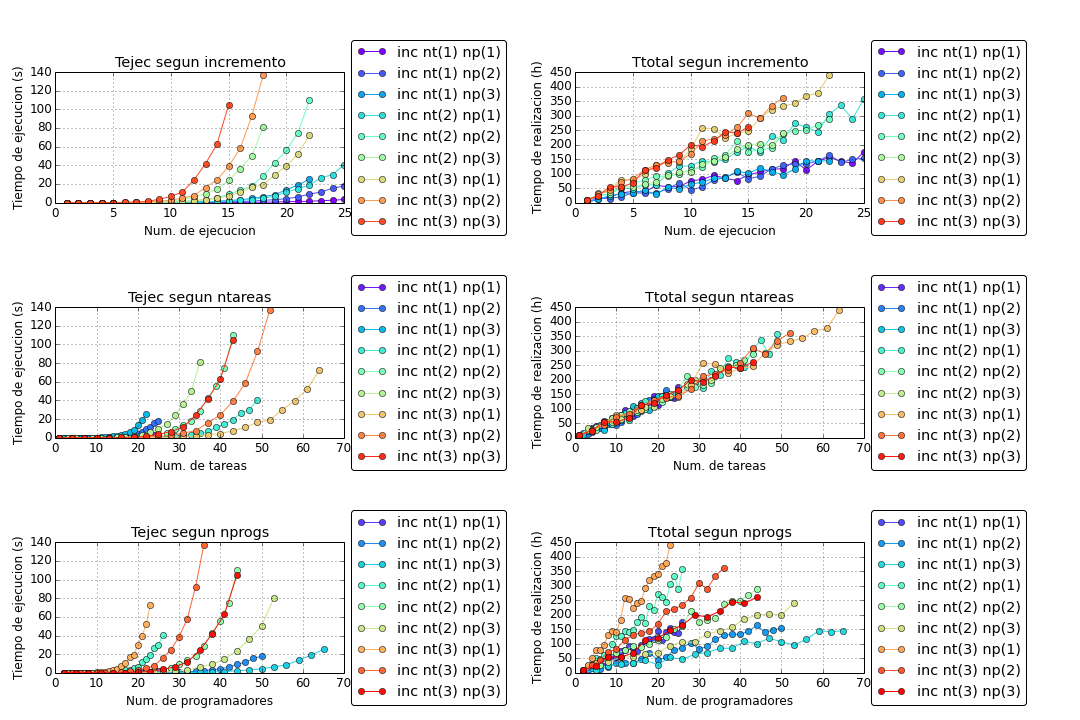
\includegraphics[height=13cm]{graph-2-1-2}
        \caption{Gráficos de los tiempos de ejecución para obtener las 
            soluciones y de los tiempos totales de desarrollo de estas en 
            función del tamaño de la entrada para la extensión 2.}
        \label{fig:extra-ext2}
    \end{figure}

\end{landscape}
}

En los gráficos de la mitad izquierda, correspondientes al tiempo de ejecución 
del \texttt{Fast Forward} para obtener la solución, se aprecia que para 
valores muy bajos la resolución es prácticamente instantánea y, a partir de 
un cierto tamaño, el tiempo de ejecución empieza a crecer de forma muy rápida 
(con los tamaños que hemos podido probar debido a las limitaciones del 
\textit{parser} del \texttt{Fast Forward} no podemos sacar conclusiones 
definitivas, pero podría tratarse de funciones polinómicas de un grado 
bastante alto, según el factor de ramificación). Esto se debe a que el 
planificador, en primera instancia, intenta encontrar una solución de forma 
rápida usando algoritmos de búsqueda local guiados por heurísticas genéricas, 
pero si no la encuentra luego procede con un algoritmo de búsqueda de tipo
\textit{best-first} que puede ser exhaustivo. Por lo tanto, para entradas 
muy pequeñas es probable que el planificador pueda hallar la respuesta con 
la primera búsqueda local pero esta ya no funcione a medida que la entrada 
crece. En este caso, como la búsqueda es prácticamente exhaustiva, el tiempo 
de ejecución depende esencialmente del factor de ramificación dado por las 
acciones del modelo.

En los gráficos de la derecha, en cambio, se representa la calidad de las 
soluciones obtenidas; es decir, la suma de las horas que los programadores 
invertirán para realizar todas las tareas asignadas en las soluciones 
obtenidas. Se aprecia claramente que, en todos los casos, este tiempo de 
resolución depende linealmente del tamaño de la entrada (básicamente del 
número de tareas). Parece muy razonable, teniendo en cuenta que los 
problemas se generan de forma aleatoria y homogénea, que el aumento del 
tiempo necesario para la realización de las tareas aumente proporcionalmente 
a la cantidad de estas (y, por lo tanto, en menor medida se aprecia en los 
gráficos una dependencia también del número de programadores, pero esto es 
porque se ha intentado mantener un cierto equilibrio entre el número de 
tareas y el número de programadores para comparar mejor la calidad de las 
soluciones). Es decir, el tiempo de resolución de las tareas depende 
linealmente del número de tareas, con una alta correlación, pero no depende 
prácticamente del número de programadores (siempre y cuando haya un número 
mínimo de programadores capaces de realizar las tareas siguiendo las 
restricciones del problema).

Se han realizado pruebas similares para todas las versiones del problema 
(las tablas y los gráficos resultantes están incluidos en los archivos 
adjuntos a este documento). El análisis de estos resultados se omite en este 
informe porque las tendencias que se aprecian en los gráficos son 
prácticamente las mismas.


